\documentclass[twoside]{book}

% Packages required by doxygen
\usepackage{fixltx2e}
\usepackage{calc}
\usepackage{doxygen}
\usepackage[export]{adjustbox} % also loads graphicx
\usepackage{graphicx}
\usepackage[utf8]{inputenc}
\usepackage{makeidx}
\usepackage{multicol}
\usepackage{multirow}
\PassOptionsToPackage{warn}{textcomp}
\usepackage{textcomp}
\usepackage[nointegrals]{wasysym}
\usepackage[table]{xcolor}

% NLS support packages
\usepackage[brazil]{babel}
% Font selection
\usepackage[T1]{fontenc}
\usepackage[scaled=.90]{helvet}
\usepackage{courier}
\usepackage{amssymb}
\usepackage{sectsty}
\renewcommand{\familydefault}{\sfdefault}
\allsectionsfont{%
  \fontseries{bc}\selectfont%
  \color{darkgray}%
}
\renewcommand{\DoxyLabelFont}{%
  \fontseries{bc}\selectfont%
  \color{darkgray}%
}
\newcommand{\+}{\discretionary{\mbox{\scriptsize$\hookleftarrow$}}{}{}}

% Page & text layout
\usepackage{geometry}
\geometry{%
  a4paper,%
  top=2.5cm,%
  bottom=2.5cm,%
  left=2.5cm,%
  right=2.5cm%
}
\tolerance=750
\hfuzz=15pt
\hbadness=750
\setlength{\emergencystretch}{15pt}
\setlength{\parindent}{0cm}
\setlength{\parskip}{0.2cm}
\makeatletter
\renewcommand{\paragraph}{%
  \@startsection{paragraph}{4}{0ex}{-1.0ex}{1.0ex}{%
    \normalfont\normalsize\bfseries\SS@parafont%
  }%
}
\renewcommand{\subparagraph}{%
  \@startsection{subparagraph}{5}{0ex}{-1.0ex}{1.0ex}{%
    \normalfont\normalsize\bfseries\SS@subparafont%
  }%
}
\makeatother

% Headers & footers
\usepackage{fancyhdr}
\pagestyle{fancyplain}
\fancyhead[LE]{\fancyplain{}{\bfseries\thepage}}
\fancyhead[CE]{\fancyplain{}{}}
\fancyhead[RE]{\fancyplain{}{\bfseries\leftmark}}
\fancyhead[LO]{\fancyplain{}{\bfseries\rightmark}}
\fancyhead[CO]{\fancyplain{}{}}
\fancyhead[RO]{\fancyplain{}{\bfseries\thepage}}
\fancyfoot[LE]{\fancyplain{}{}}
\fancyfoot[CE]{\fancyplain{}{}}
\fancyfoot[RE]{\fancyplain{}{\bfseries\scriptsize Gerado em Sexta, 20 de Maio de 2016 21\+:41\+:54 para „\+Processo\+Usuario“ por Doxygen }}
\fancyfoot[LO]{\fancyplain{}{\bfseries\scriptsize Gerado em Sexta, 20 de Maio de 2016 21\+:41\+:54 para „\+Processo\+Usuario“ por Doxygen }}
\fancyfoot[CO]{\fancyplain{}{}}
\fancyfoot[RO]{\fancyplain{}{}}
\renewcommand{\footrulewidth}{0.4pt}
\renewcommand{\chaptermark}[1]{%
  \markboth{#1}{}%
}
\renewcommand{\sectionmark}[1]{%
  \markright{\thesection\ #1}%
}

% Indices & bibliography
\usepackage{natbib}
\usepackage[titles]{tocloft}
\setcounter{tocdepth}{3}
\setcounter{secnumdepth}{5}
\makeindex

% Hyperlinks (required, but should be loaded last)
\usepackage{ifpdf}
\ifpdf
  \usepackage[pdftex,pagebackref=true]{hyperref}
\else
  \usepackage[ps2pdf,pagebackref=true]{hyperref}
\fi
\hypersetup{%
  colorlinks=true,%
  linkcolor=blue,%
  citecolor=blue,%
  unicode%
}

% Custom commands
\newcommand{\clearemptydoublepage}{%
  \newpage{\pagestyle{empty}\cleardoublepage}%
}


%===== C O N T E N T S =====

\begin{document}

% Titlepage & ToC
\hypersetup{pageanchor=false,
             bookmarks=true,
             bookmarksnumbered=true,
             pdfencoding=unicode
            }
\pagenumbering{roman}
\begin{titlepage}
\vspace*{7cm}
\begin{center}%
{\Large „\+Processo\+Usuario“ }\\
\vspace*{1cm}
{\large Gerado por Doxygen 1.8.10}\\
\vspace*{0.5cm}
{\small Sexta, 20 de Maio de 2016 21:41:54}\\
\end{center}
\end{titlepage}
\clearemptydoublepage
\tableofcontents
\clearemptydoublepage
\pagenumbering{arabic}
\hypersetup{pageanchor=true}

%--- Begin generated contents ---
\chapter{Índice das Estruturas de Dados}
\section{Estruturas de Dados}
Aqui estão as estruturas de dados, uniões e suas respectivas descrições\+:\begin{DoxyCompactList}
\item\contentsline{section}{\hyperlink{structmensagem}{mensagem} \\*Estrutura de mensagem }{\pageref{structmensagem}}{}
\end{DoxyCompactList}

\chapter{Índice dos Arquivos}
\section{Lista de Arquivos}
Esta é a lista de todos os arquivos e suas respectivas descrições\+:\begin{DoxyCompactList}
\item\contentsline{section}{include/\hyperlink{_e___m_e_n_s_a_g_e_m_8h}{E\+\_\+\+M\+E\+N\+S\+A\+G\+E\+M.\+h} \\*Interface de estrutura de mensagens }{\pageref{_e___m_e_n_s_a_g_e_m_8h}}{}
\item\contentsline{section}{include/\hyperlink{_e___s_e_m_a_f_o_r_o_8h}{E\+\_\+\+S\+E\+M\+A\+F\+O\+R\+O.\+h} \\*Interface dos semaforos de Dijkstra }{\pageref{_e___s_e_m_a_f_o_r_o_8h}}{}
\item\contentsline{section}{include/\hyperlink{_e___t_a_b_f_r_a_m_e_s_8h}{E\+\_\+\+T\+A\+B\+F\+R\+A\+M\+E\+S.\+h} \\*Interface de estrutura da tabela de frames }{\pageref{_e___t_a_b_f_r_a_m_e_s_8h}}{}
\item\contentsline{section}{include/\hyperlink{_i___a_l_o_c_p_a_g_8h}{I\+\_\+\+A\+L\+O\+C\+P\+A\+G.\+h} \\*Interface do alocador de paginas }{\pageref{_i___a_l_o_c_p_a_g_8h}}{}
\item\contentsline{section}{include/\hyperlink{_i___s_u_b_s_p_a_g_8h}{I\+\_\+\+S\+U\+B\+S\+P\+A\+G.\+h} \\*Interface do substituidor de paginas }{\pageref{_i___s_u_b_s_p_a_g_8h}}{}
\item\contentsline{section}{src/\hyperlink{_m___a_l_o_c_p_a_g_8c}{M\+\_\+\+A\+L\+O\+C\+P\+A\+G.\+c} \\*Modulo do alocador de paginas }{\pageref{_m___a_l_o_c_p_a_g_8c}}{}
\item\contentsline{section}{src/\hyperlink{_m___m_e_n_s_a_g_e_m_8c}{M\+\_\+\+M\+E\+N\+S\+A\+G\+E\+M.\+c} }{\pageref{_m___m_e_n_s_a_g_e_m_8c}}{}
\item\contentsline{section}{src/\hyperlink{_m___s_e_m_a_f_o_r_o_8c}{M\+\_\+\+S\+E\+M\+A\+F\+O\+R\+O.\+c} \\*Modulo dos semaforos de Dijkstra }{\pageref{_m___s_e_m_a_f_o_r_o_8c}}{}
\item\contentsline{section}{src/\hyperlink{_m___s_e_r_v_m_e_m_8c}{M\+\_\+\+S\+E\+R\+V\+M\+E\+M.\+c} \\*Modulo de Inicializacao do servidor de memória }{\pageref{_m___s_e_r_v_m_e_m_8c}}{}
\item\contentsline{section}{src/\hyperlink{_m___s_u_b_s_p_a_g_8c}{M\+\_\+\+S\+U\+B\+S\+P\+A\+G.\+c} \\*Modulo do substituidor de paginas }{\pageref{_m___s_u_b_s_p_a_g_8c}}{}
\item\contentsline{section}{src/\hyperlink{_m___t_a_b_f_r_a_m_e_s_8c}{M\+\_\+\+T\+A\+B\+F\+R\+A\+M\+E\+S.\+c} \\*Modulo de estrutura de tabela de frames }{\pageref{_m___t_a_b_f_r_a_m_e_s_8c}}{}
\end{DoxyCompactList}

\chapter{Estruturas}
\hypertarget{structmensagem}{}\section{Referência da Estrutura mensagem}
\label{structmensagem}\index{mensagem@{mensagem}}


Estrutura de mensagem.  




{\ttfamily \#include $<$E\+\_\+\+M\+E\+N\+S\+A\+G\+E\+M.\+h$>$}

\subsection*{Campos de Dados}
\begin{DoxyCompactItemize}
\item 
long \hyperlink{structmensagem_a0c2d7145cc186c97a721bf6cc00576be}{pid}
\item 
int \hyperlink{structmensagem_ae517cd66c376c75e1a242660e3892184}{num}
\begin{DoxyCompactList}\small\item\em Numero da pagina ou frame. \end{DoxyCompactList}\end{DoxyCompactItemize}


\subsection{Descrição Detalhada}
Estrutura de mensagem. 

Estrura que representa uma mensagem de comunicacao entre processos. 

\subsection{Campos}
\hypertarget{structmensagem_ae517cd66c376c75e1a242660e3892184}{}\index{mensagem@{mensagem}!num@{num}}
\index{num@{num}!mensagem@{mensagem}}
\subsubsection[{num}]{\setlength{\rightskip}{0pt plus 5cm}int mensagem\+::num}\label{structmensagem_ae517cd66c376c75e1a242660e3892184}


Numero da pagina ou frame. 

\hypertarget{structmensagem_a0c2d7145cc186c97a721bf6cc00576be}{}\index{mensagem@{mensagem}!pid@{pid}}
\index{pid@{pid}!mensagem@{mensagem}}
\subsubsection[{pid}]{\setlength{\rightskip}{0pt plus 5cm}long mensagem\+::pid}\label{structmensagem_a0c2d7145cc186c97a721bf6cc00576be}


A documentação para esta estrutura foi gerada a partir do seguinte arquivo\+:\begin{DoxyCompactItemize}
\item 
include/\hyperlink{_e___m_e_n_s_a_g_e_m_8h}{E\+\_\+\+M\+E\+N\+S\+A\+G\+E\+M.\+h}\end{DoxyCompactItemize}

\chapter{Arquivos}
\hypertarget{_e___m_e_n_s_a_g_e_m_8h}{}\section{Referência do Arquivo include/\+E\+\_\+\+M\+E\+N\+S\+A\+G\+E\+M.h}
\label{_e___m_e_n_s_a_g_e_m_8h}\index{include/\+E\+\_\+\+M\+E\+N\+S\+A\+G\+E\+M.\+h@{include/\+E\+\_\+\+M\+E\+N\+S\+A\+G\+E\+M.\+h}}


Interface de estrutura de mensagens.  


{\ttfamily \#include $<$stdlib.\+h$>$}\\*
{\ttfamily \#include $<$errno.\+h$>$}\\*
{\ttfamily \#include $<$sys/types.\+h$>$}\\*
{\ttfamily \#include $<$sys/ipc.\+h$>$}\\*
{\ttfamily \#include $<$sys/msg.\+h$>$}\\*
Gráfico de dependência de inclusões para E\+\_\+\+M\+E\+N\+S\+A\+G\+E\+M.\+h\+:
\nopagebreak
\begin{figure}[H]
\begin{center}
\leavevmode
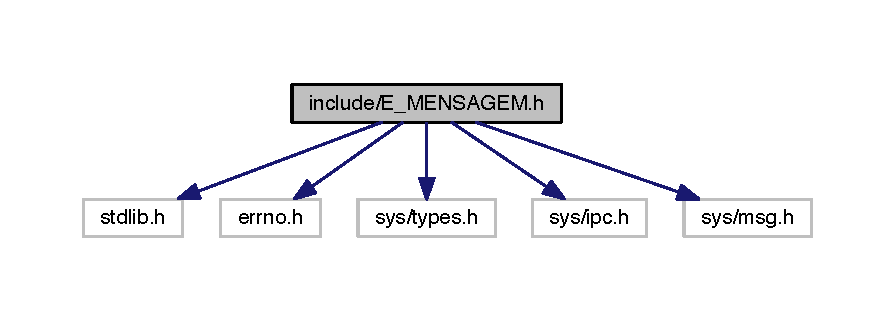
\includegraphics[width=350pt]{_e___m_e_n_s_a_g_e_m_8h__incl}
\end{center}
\end{figure}
Este grafo mostra quais arquivos estão direta ou indiretamente relacionados com este arquivo\+:
\nopagebreak
\begin{figure}[H]
\begin{center}
\leavevmode
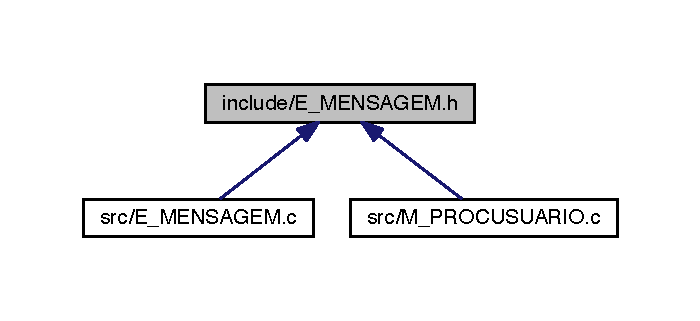
\includegraphics[width=336pt]{_e___m_e_n_s_a_g_e_m_8h__dep__incl}
\end{center}
\end{figure}
\subsection*{Estruturas de Dados}
\begin{DoxyCompactItemize}
\item 
struct \hyperlink{structmensagem}{mensagem}
\begin{DoxyCompactList}\small\item\em Estrutura de mensagem. \end{DoxyCompactList}\end{DoxyCompactItemize}
\subsection*{Definições e Macros}
\begin{DoxyCompactItemize}
\item 
\#define \hyperlink{_e___m_e_n_s_a_g_e_m_8h_ae4ad4682bcea787f40f19afc2c3dc907}{E\+X\+T6}~extern
\item 
\#define \hyperlink{_e___m_e_n_s_a_g_e_m_8h_a430964ddbf255bb5305cb4d183f7aeaa}{K\+E\+Y\+\_\+\+T0}~0x398801
\begin{DoxyCompactList}\small\item\em Chave para a fila de mensagens do processo de alocacao de memoria. \end{DoxyCompactList}\item 
\#define \hyperlink{_e___m_e_n_s_a_g_e_m_8h_ad839b4de8d1726d14f7aa96520d63a75}{K\+E\+Y\+\_\+\+T1}~0x539712
\begin{DoxyCompactList}\small\item\em Chave para a fila de mensagens para notificacao dos processo de usuario. \end{DoxyCompactList}\end{DoxyCompactItemize}
\subsection*{Definições de Tipos}
\begin{DoxyCompactItemize}
\item 
typedef struct \hyperlink{structmensagem}{mensagem} \hyperlink{_e___m_e_n_s_a_g_e_m_8h_a7f28ef2afbad397da434a1a718a4b45a}{Mensagem}
\begin{DoxyCompactList}\small\item\em Estrutura de mensagem. \end{DoxyCompactList}\end{DoxyCompactItemize}
\subsection*{Funções}
\begin{DoxyCompactItemize}
\item 
\hyperlink{_e___m_e_n_s_a_g_e_m_8h_ae4ad4682bcea787f40f19afc2c3dc907}{E\+X\+T6} \hyperlink{_e___m_e_n_s_a_g_e_m_8h_a7f28ef2afbad397da434a1a718a4b45a}{Mensagem} $\ast$ \hyperlink{_e___m_e_n_s_a_g_e_m_8h_a681f7d0fe37fb0c9956243abc7abd9b7}{inicializa\+Mensagem} ()
\end{DoxyCompactItemize}


\subsection{Descrição Detalhada}
Interface de estrutura de mensagens. 

Interface responsavel pela definicao da estrutura de mensagens utilizadas na fila de mensagens para a comunicação entre processos. 

\subsection{Definições e macros}
\hypertarget{_e___m_e_n_s_a_g_e_m_8h_ae4ad4682bcea787f40f19afc2c3dc907}{}\index{E\+\_\+\+M\+E\+N\+S\+A\+G\+E\+M.\+h@{E\+\_\+\+M\+E\+N\+S\+A\+G\+E\+M.\+h}!E\+X\+T6@{E\+X\+T6}}
\index{E\+X\+T6@{E\+X\+T6}!E\+\_\+\+M\+E\+N\+S\+A\+G\+E\+M.\+h@{E\+\_\+\+M\+E\+N\+S\+A\+G\+E\+M.\+h}}
\subsubsection[{E\+X\+T6}]{\setlength{\rightskip}{0pt plus 5cm}\#define E\+X\+T6~extern}\label{_e___m_e_n_s_a_g_e_m_8h_ae4ad4682bcea787f40f19afc2c3dc907}
\hypertarget{_e___m_e_n_s_a_g_e_m_8h_a430964ddbf255bb5305cb4d183f7aeaa}{}\index{E\+\_\+\+M\+E\+N\+S\+A\+G\+E\+M.\+h@{E\+\_\+\+M\+E\+N\+S\+A\+G\+E\+M.\+h}!K\+E\+Y\+\_\+\+T0@{K\+E\+Y\+\_\+\+T0}}
\index{K\+E\+Y\+\_\+\+T0@{K\+E\+Y\+\_\+\+T0}!E\+\_\+\+M\+E\+N\+S\+A\+G\+E\+M.\+h@{E\+\_\+\+M\+E\+N\+S\+A\+G\+E\+M.\+h}}
\subsubsection[{K\+E\+Y\+\_\+\+T0}]{\setlength{\rightskip}{0pt plus 5cm}\#define K\+E\+Y\+\_\+\+T0~0x398801}\label{_e___m_e_n_s_a_g_e_m_8h_a430964ddbf255bb5305cb4d183f7aeaa}


Chave para a fila de mensagens do processo de alocacao de memoria. 

\hypertarget{_e___m_e_n_s_a_g_e_m_8h_ad839b4de8d1726d14f7aa96520d63a75}{}\index{E\+\_\+\+M\+E\+N\+S\+A\+G\+E\+M.\+h@{E\+\_\+\+M\+E\+N\+S\+A\+G\+E\+M.\+h}!K\+E\+Y\+\_\+\+T1@{K\+E\+Y\+\_\+\+T1}}
\index{K\+E\+Y\+\_\+\+T1@{K\+E\+Y\+\_\+\+T1}!E\+\_\+\+M\+E\+N\+S\+A\+G\+E\+M.\+h@{E\+\_\+\+M\+E\+N\+S\+A\+G\+E\+M.\+h}}
\subsubsection[{K\+E\+Y\+\_\+\+T1}]{\setlength{\rightskip}{0pt plus 5cm}\#define K\+E\+Y\+\_\+\+T1~0x539712}\label{_e___m_e_n_s_a_g_e_m_8h_ad839b4de8d1726d14f7aa96520d63a75}


Chave para a fila de mensagens para notificacao dos processo de usuario. 



\subsection{Definições dos tipos}
\hypertarget{_e___m_e_n_s_a_g_e_m_8h_a7f28ef2afbad397da434a1a718a4b45a}{}\index{E\+\_\+\+M\+E\+N\+S\+A\+G\+E\+M.\+h@{E\+\_\+\+M\+E\+N\+S\+A\+G\+E\+M.\+h}!Mensagem@{Mensagem}}
\index{Mensagem@{Mensagem}!E\+\_\+\+M\+E\+N\+S\+A\+G\+E\+M.\+h@{E\+\_\+\+M\+E\+N\+S\+A\+G\+E\+M.\+h}}
\subsubsection[{Mensagem}]{\setlength{\rightskip}{0pt plus 5cm}typedef struct {\bf mensagem}  {\bf Mensagem}}\label{_e___m_e_n_s_a_g_e_m_8h_a7f28ef2afbad397da434a1a718a4b45a}


Estrutura de mensagem. 

Estrura que representa uma mensagem de comunicacao entre processos. 

\subsection{Funções}
\hypertarget{_e___m_e_n_s_a_g_e_m_8h_a681f7d0fe37fb0c9956243abc7abd9b7}{}\index{E\+\_\+\+M\+E\+N\+S\+A\+G\+E\+M.\+h@{E\+\_\+\+M\+E\+N\+S\+A\+G\+E\+M.\+h}!inicializa\+Mensagem@{inicializa\+Mensagem}}
\index{inicializa\+Mensagem@{inicializa\+Mensagem}!E\+\_\+\+M\+E\+N\+S\+A\+G\+E\+M.\+h@{E\+\_\+\+M\+E\+N\+S\+A\+G\+E\+M.\+h}}
\subsubsection[{inicializa\+Mensagem()}]{\setlength{\rightskip}{0pt plus 5cm}{\bf E\+X\+T6} {\bf Mensagem}$\ast$ inicializa\+Mensagem (
\begin{DoxyParamCaption}
{}
\end{DoxyParamCaption}
)}\label{_e___m_e_n_s_a_g_e_m_8h_a681f7d0fe37fb0c9956243abc7abd9b7}
Metodo responsavel por inicializar e retornar uma estrutura de mensagem

\begin{DoxyReturn}{Retorna}
Estrutura de mensagem inicializada 
\end{DoxyReturn}

\hypertarget{_e___m_e_n_s_a_g_e_m_8c}{}\section{Referência do Arquivo src/\+E\+\_\+\+M\+E\+N\+S\+A\+G\+E\+M.c}
\label{_e___m_e_n_s_a_g_e_m_8c}\index{src/\+E\+\_\+\+M\+E\+N\+S\+A\+G\+E\+M.\+c@{src/\+E\+\_\+\+M\+E\+N\+S\+A\+G\+E\+M.\+c}}
{\ttfamily \#include \char`\"{}../include/\+E\+\_\+\+M\+E\+N\+S\+A\+G\+E\+M.\+h\char`\"{}}\\*
Gráfico de dependência de inclusões para E\+\_\+\+M\+E\+N\+S\+A\+G\+E\+M.\+c\+:
\nopagebreak
\begin{figure}[H]
\begin{center}
\leavevmode
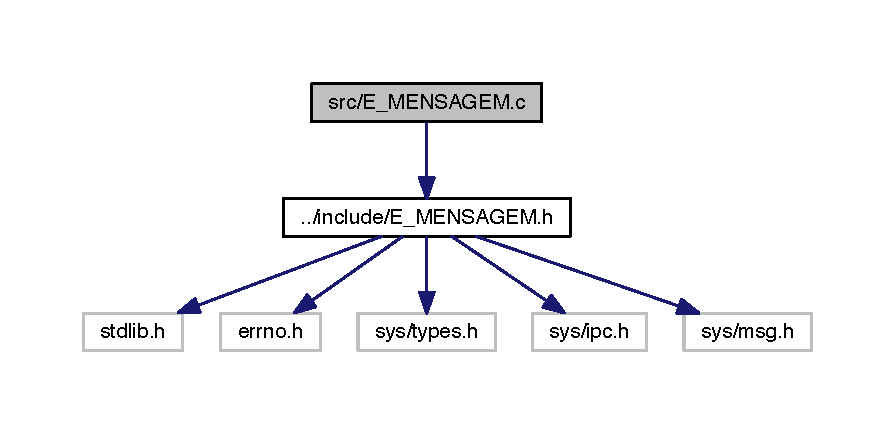
\includegraphics[width=350pt]{_e___m_e_n_s_a_g_e_m_8c__incl}
\end{center}
\end{figure}
\subsection*{Definições e Macros}
\begin{DoxyCompactItemize}
\item 
\#define \hyperlink{_e___m_e_n_s_a_g_e_m_8c_a590361aaef63faec2f5ea7090da043e3}{M\+\_\+\+M\+E\+N\+S\+A\+G\+E\+M}
\end{DoxyCompactItemize}
\subsection*{Funções}
\begin{DoxyCompactItemize}
\item 
\hyperlink{_e___m_e_n_s_a_g_e_m_8h_a7f28ef2afbad397da434a1a718a4b45a}{Mensagem} $\ast$ \hyperlink{_e___m_e_n_s_a_g_e_m_8c_a32cd4747ae5357b3b75593a7e1963098}{inicializa\+Mensagem} ()
\end{DoxyCompactItemize}


\subsection{Definições e macros}
\hypertarget{_e___m_e_n_s_a_g_e_m_8c_a590361aaef63faec2f5ea7090da043e3}{}\index{E\+\_\+\+M\+E\+N\+S\+A\+G\+E\+M.\+c@{E\+\_\+\+M\+E\+N\+S\+A\+G\+E\+M.\+c}!M\+\_\+\+M\+E\+N\+S\+A\+G\+E\+M@{M\+\_\+\+M\+E\+N\+S\+A\+G\+E\+M}}
\index{M\+\_\+\+M\+E\+N\+S\+A\+G\+E\+M@{M\+\_\+\+M\+E\+N\+S\+A\+G\+E\+M}!E\+\_\+\+M\+E\+N\+S\+A\+G\+E\+M.\+c@{E\+\_\+\+M\+E\+N\+S\+A\+G\+E\+M.\+c}}
\subsubsection[{M\+\_\+\+M\+E\+N\+S\+A\+G\+E\+M}]{\setlength{\rightskip}{0pt plus 5cm}\#define M\+\_\+\+M\+E\+N\+S\+A\+G\+E\+M}\label{_e___m_e_n_s_a_g_e_m_8c_a590361aaef63faec2f5ea7090da043e3}


\subsection{Funções}
\hypertarget{_e___m_e_n_s_a_g_e_m_8c_a32cd4747ae5357b3b75593a7e1963098}{}\index{E\+\_\+\+M\+E\+N\+S\+A\+G\+E\+M.\+c@{E\+\_\+\+M\+E\+N\+S\+A\+G\+E\+M.\+c}!inicializa\+Mensagem@{inicializa\+Mensagem}}
\index{inicializa\+Mensagem@{inicializa\+Mensagem}!E\+\_\+\+M\+E\+N\+S\+A\+G\+E\+M.\+c@{E\+\_\+\+M\+E\+N\+S\+A\+G\+E\+M.\+c}}
\subsubsection[{inicializa\+Mensagem()}]{\setlength{\rightskip}{0pt plus 5cm}{\bf Mensagem}$\ast$ inicializa\+Mensagem (
\begin{DoxyParamCaption}
{}
\end{DoxyParamCaption}
)}\label{_e___m_e_n_s_a_g_e_m_8c_a32cd4747ae5357b3b75593a7e1963098}
Metodo responsavel por inicializar e retornar uma estrutura de mensagem

\begin{DoxyReturn}{Retorna}
Estrutura de mensagem inicializada 
\end{DoxyReturn}

\hypertarget{_m___p_r_o_c_u_s_u_a_r_i_o_8c}{}\section{Referência do Arquivo src/\+M\+\_\+\+P\+R\+O\+C\+U\+S\+U\+A\+R\+I\+O.c}
\label{_m___p_r_o_c_u_s_u_a_r_i_o_8c}\index{src/\+M\+\_\+\+P\+R\+O\+C\+U\+S\+U\+A\+R\+I\+O.\+c@{src/\+M\+\_\+\+P\+R\+O\+C\+U\+S\+U\+A\+R\+I\+O.\+c}}


Modulo do processo de usuario.  


{\ttfamily \#include $<$stdio.\+h$>$}\\*
{\ttfamily \#include $<$string.\+h$>$}\\*
{\ttfamily \#include $<$unistd.\+h$>$}\\*
{\ttfamily \#include $<$signal.\+h$>$}\\*
{\ttfamily \#include \char`\"{}../include/\+E\+\_\+\+M\+E\+N\+S\+A\+G\+E\+M.\+h\char`\"{}}\\*
Gráfico de dependência de inclusões para M\+\_\+\+P\+R\+O\+C\+U\+S\+U\+A\+R\+I\+O.\+c\+:
\nopagebreak
\begin{figure}[H]
\begin{center}
\leavevmode
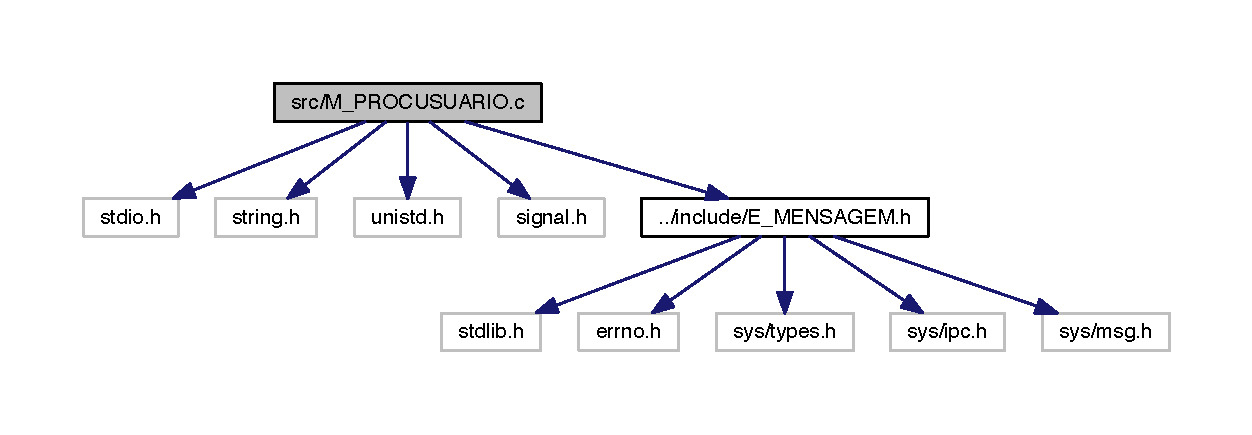
\includegraphics[width=350pt]{_m___p_r_o_c_u_s_u_a_r_i_o_8c__incl}
\end{center}
\end{figure}
\subsection*{Definições e Macros}
\begin{DoxyCompactItemize}
\item 
\#define \hyperlink{_m___p_r_o_c_u_s_u_a_r_i_o_8c_a810c5b751df5bb30588613ed91095129}{N\+P\+R\+O\+C}~10
\begin{DoxyCompactList}\small\item\em Numero total de processos de usuario. \end{DoxyCompactList}\end{DoxyCompactItemize}
\subsection*{Funções}
\begin{DoxyCompactItemize}
\item 
int \hyperlink{_m___p_r_o_c_u_s_u_a_r_i_o_8c_ac0f2228420376f4db7e1274f2b41667c}{main} (int argc, const char $\ast$argv\mbox{[}$\,$\mbox{]})
\end{DoxyCompactItemize}
\subsection*{Variáveis}
\begin{DoxyCompactItemize}
\item 
int \hyperlink{_m___p_r_o_c_u_s_u_a_r_i_o_8c_af500917c052066b40cf47f96b43c607b}{pid}
\begin{DoxyCompactList}\small\item\em id do processo atual \end{DoxyCompactList}\item 
int \hyperlink{_m___p_r_o_c_u_s_u_a_r_i_o_8c_a88878a2af8d822b257daf3145a09b725}{msg\+\_\+aloc\+\_\+id}
\begin{DoxyCompactList}\small\item\em id das filas de mensagem de entrada do alocador \end{DoxyCompactList}\item 
int \hyperlink{_m___p_r_o_c_u_s_u_a_r_i_o_8c_ae57050834a3b1770e0e855e42f4ad41d}{msg\+\_\+usu\+\_\+id}
\begin{DoxyCompactList}\small\item\em id das filas de mensagem de notificacao dos usuarios \end{DoxyCompactList}\end{DoxyCompactItemize}


\subsection{Descrição Detalhada}
Modulo do processo de usuario. 

Modulo responsavel por implementar os metodos relacionados a criacao de N processos de usuarios, em que cada um realiza uma chamada a primitiva referencia\+\_\+pagina(i), onde i eh o numero da pagina. Essas paginas a serem referenciadas por um processo n estao no arquivo pag\+\_\+processo\+\_\+n. 

\subsection{Definições e macros}
\hypertarget{_m___p_r_o_c_u_s_u_a_r_i_o_8c_a810c5b751df5bb30588613ed91095129}{}\index{M\+\_\+\+P\+R\+O\+C\+U\+S\+U\+A\+R\+I\+O.\+c@{M\+\_\+\+P\+R\+O\+C\+U\+S\+U\+A\+R\+I\+O.\+c}!N\+P\+R\+O\+C@{N\+P\+R\+O\+C}}
\index{N\+P\+R\+O\+C@{N\+P\+R\+O\+C}!M\+\_\+\+P\+R\+O\+C\+U\+S\+U\+A\+R\+I\+O.\+c@{M\+\_\+\+P\+R\+O\+C\+U\+S\+U\+A\+R\+I\+O.\+c}}
\subsubsection[{N\+P\+R\+O\+C}]{\setlength{\rightskip}{0pt plus 5cm}\#define N\+P\+R\+O\+C~10}\label{_m___p_r_o_c_u_s_u_a_r_i_o_8c_a810c5b751df5bb30588613ed91095129}


Numero total de processos de usuario. 



\subsection{Funções}
\hypertarget{_m___p_r_o_c_u_s_u_a_r_i_o_8c_ac0f2228420376f4db7e1274f2b41667c}{}\index{M\+\_\+\+P\+R\+O\+C\+U\+S\+U\+A\+R\+I\+O.\+c@{M\+\_\+\+P\+R\+O\+C\+U\+S\+U\+A\+R\+I\+O.\+c}!main@{main}}
\index{main@{main}!M\+\_\+\+P\+R\+O\+C\+U\+S\+U\+A\+R\+I\+O.\+c@{M\+\_\+\+P\+R\+O\+C\+U\+S\+U\+A\+R\+I\+O.\+c}}
\subsubsection[{main(int argc, const char $\ast$argv[])}]{\setlength{\rightskip}{0pt plus 5cm}int main (
\begin{DoxyParamCaption}
\item[{int}]{argc, }
\item[{const char $\ast$}]{argv\mbox{[}$\,$\mbox{]}}
\end{DoxyParamCaption}
)}\label{_m___p_r_o_c_u_s_u_a_r_i_o_8c_ac0f2228420376f4db7e1274f2b41667c}
Metodo inicial do sistema 

Este é o diagrama das funções utilizadas por esta função\+:
\nopagebreak
\begin{figure}[H]
\begin{center}
\leavevmode
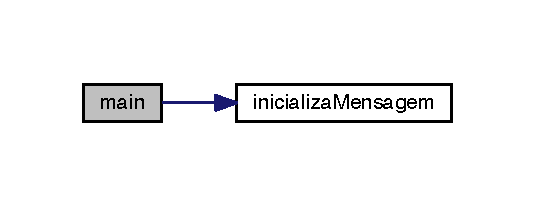
\includegraphics[width=257pt]{_m___p_r_o_c_u_s_u_a_r_i_o_8c_ac0f2228420376f4db7e1274f2b41667c_cgraph}
\end{center}
\end{figure}




\subsection{Variáveis}
\hypertarget{_m___p_r_o_c_u_s_u_a_r_i_o_8c_a88878a2af8d822b257daf3145a09b725}{}\index{M\+\_\+\+P\+R\+O\+C\+U\+S\+U\+A\+R\+I\+O.\+c@{M\+\_\+\+P\+R\+O\+C\+U\+S\+U\+A\+R\+I\+O.\+c}!msg\+\_\+aloc\+\_\+id@{msg\+\_\+aloc\+\_\+id}}
\index{msg\+\_\+aloc\+\_\+id@{msg\+\_\+aloc\+\_\+id}!M\+\_\+\+P\+R\+O\+C\+U\+S\+U\+A\+R\+I\+O.\+c@{M\+\_\+\+P\+R\+O\+C\+U\+S\+U\+A\+R\+I\+O.\+c}}
\subsubsection[{msg\+\_\+aloc\+\_\+id}]{\setlength{\rightskip}{0pt plus 5cm}int msg\+\_\+aloc\+\_\+id}\label{_m___p_r_o_c_u_s_u_a_r_i_o_8c_a88878a2af8d822b257daf3145a09b725}


id das filas de mensagem de entrada do alocador 

\hypertarget{_m___p_r_o_c_u_s_u_a_r_i_o_8c_ae57050834a3b1770e0e855e42f4ad41d}{}\index{M\+\_\+\+P\+R\+O\+C\+U\+S\+U\+A\+R\+I\+O.\+c@{M\+\_\+\+P\+R\+O\+C\+U\+S\+U\+A\+R\+I\+O.\+c}!msg\+\_\+usu\+\_\+id@{msg\+\_\+usu\+\_\+id}}
\index{msg\+\_\+usu\+\_\+id@{msg\+\_\+usu\+\_\+id}!M\+\_\+\+P\+R\+O\+C\+U\+S\+U\+A\+R\+I\+O.\+c@{M\+\_\+\+P\+R\+O\+C\+U\+S\+U\+A\+R\+I\+O.\+c}}
\subsubsection[{msg\+\_\+usu\+\_\+id}]{\setlength{\rightskip}{0pt plus 5cm}int msg\+\_\+usu\+\_\+id}\label{_m___p_r_o_c_u_s_u_a_r_i_o_8c_ae57050834a3b1770e0e855e42f4ad41d}


id das filas de mensagem de notificacao dos usuarios 

\hypertarget{_m___p_r_o_c_u_s_u_a_r_i_o_8c_af500917c052066b40cf47f96b43c607b}{}\index{M\+\_\+\+P\+R\+O\+C\+U\+S\+U\+A\+R\+I\+O.\+c@{M\+\_\+\+P\+R\+O\+C\+U\+S\+U\+A\+R\+I\+O.\+c}!pid@{pid}}
\index{pid@{pid}!M\+\_\+\+P\+R\+O\+C\+U\+S\+U\+A\+R\+I\+O.\+c@{M\+\_\+\+P\+R\+O\+C\+U\+S\+U\+A\+R\+I\+O.\+c}}
\subsubsection[{pid}]{\setlength{\rightskip}{0pt plus 5cm}int pid}\label{_m___p_r_o_c_u_s_u_a_r_i_o_8c_af500917c052066b40cf47f96b43c607b}


id do processo atual 


%--- End generated contents ---

% Index
\backmatter
\newpage
\phantomsection
\clearemptydoublepage
\addcontentsline{toc}{chapter}{Índice}
\printindex

\end{document}
